% Anatomy of a Job — real-time task timing diagram
% Compile:  pdflatex anatomy_job.tex  &&  dvisvgm --pdf anatomy_job.pdf
\documentclass[border=3pt]{standalone}
\usepackage{lmodern}
\usepackage{tikz}
\usetikzlibrary{arrows.meta,decorations.pathreplacing}

\definecolor{kmblue}{HTML}{003874}
\definecolor{kmgold}{HTML}{BA9224}
\definecolor{rtgreen}{HTML}{1F9D55}
\definecolor{rtred}{HTML}{E3342F}
\definecolor{axgray}{HTML}{888888}
\definecolor{dkgray}{HTML}{555555}

\begin{document}
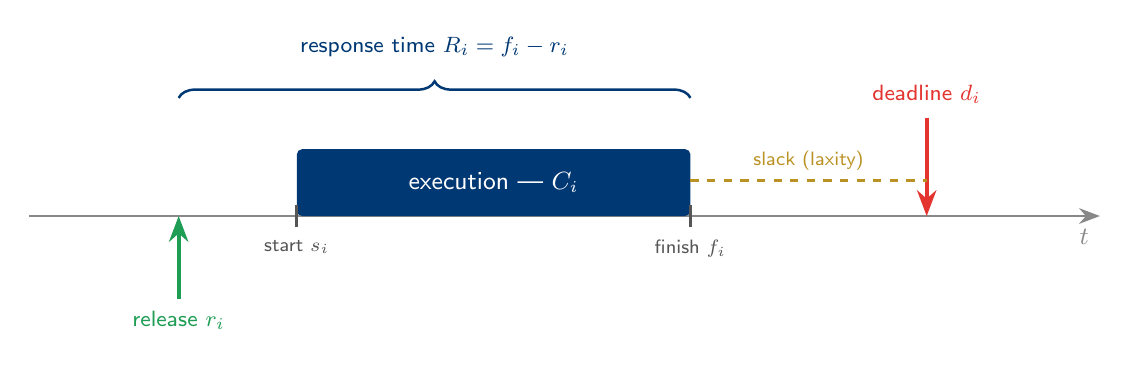
\begin{tikzpicture}[>=Stealth,font=\sffamily,x=1cm,y=1cm]

  % --- timeline axis ---
  \draw[axgray,line width=1pt,->] (-0.4,0) -- (13.2,0);
  \node[axgray,font=\sffamily\small,below] at (13.0,-0.04) {$t$};

  % --- execution block ---
  \fill[kmblue,rounded corners=2pt] (3,0) rectangle (8,0.85);
  \node[white,font=\sffamily\small] at (5.5,0.425) {execution --- $C_i$};

  % --- response-time brace ---
  \draw[kmblue,line width=0.9pt,decorate,
        decoration={brace,amplitude=6pt}] (1.5,1.5) -- (8,1.5);
  \node[kmblue,font=\sffamily\footnotesize] at (4.75,2.15)
        {response time $R_i = f_i - r_i$};

  % --- release arrow (up) ---
  \draw[rtgreen,line width=1.4pt,->] (1.5,-1.05) -- (1.5,0);
  \node[rtgreen,font=\sffamily\footnotesize,below] at (1.5,-1.08)
        {release $r_i$};

  % --- deadline arrow (down) ---
  \draw[rtred,line width=1.4pt,->] (11,1.25) -- (11,0);
  \node[rtred,font=\sffamily\footnotesize,above] at (11,1.3)
        {deadline $d_i$};

  % --- start / finish ticks ---
  \draw[dkgray,line width=1pt] (3,-0.14) -- (3,0.14);
  \node[dkgray,font=\sffamily\scriptsize,below] at (3,-0.18) {start $s_i$};
  \draw[dkgray,line width=1pt] (8,-0.14) -- (8,0.14);
  \node[dkgray,font=\sffamily\scriptsize,below] at (8,-0.18) {finish $f_i$};

  % --- slack / laxity ---
  \draw[kmgold,line width=1.1pt,dashed] (8,0.45) -- (11,0.45);
  \node[kmgold,font=\sffamily\scriptsize,above] at (9.5,0.45)
        {slack (laxity)};

\end{tikzpicture}
\end{document}
